\documentclass[11pt,letter]{article}\usepackage[]{graphicx}\usepackage[]{color}
%% maxwidth is the original width if it is less than linewidth
%% otherwise use linewidth (to make sure the graphics do not exceed the margin)
\makeatletter
\def\maxwidth{ %
  \ifdim\Gin@nat@width>\linewidth
    \linewidth
  \else
    \Gin@nat@width
  \fi
}
\makeatother

\definecolor{fgcolor}{rgb}{0.345, 0.345, 0.345}
\newcommand{\hlnum}[1]{\textcolor[rgb]{0.686,0.059,0.569}{#1}}%
\newcommand{\hlstr}[1]{\textcolor[rgb]{0.192,0.494,0.8}{#1}}%
\newcommand{\hlcom}[1]{\textcolor[rgb]{0.678,0.584,0.686}{\textit{#1}}}%
\newcommand{\hlopt}[1]{\textcolor[rgb]{0,0,0}{#1}}%
\newcommand{\hlstd}[1]{\textcolor[rgb]{0.345,0.345,0.345}{#1}}%
\newcommand{\hlkwa}[1]{\textcolor[rgb]{0.161,0.373,0.58}{\textbf{#1}}}%
\newcommand{\hlkwb}[1]{\textcolor[rgb]{0.69,0.353,0.396}{#1}}%
\newcommand{\hlkwc}[1]{\textcolor[rgb]{0.333,0.667,0.333}{#1}}%
\newcommand{\hlkwd}[1]{\textcolor[rgb]{0.737,0.353,0.396}{\textbf{#1}}}%
\let\hlipl\hlkwb

\usepackage{framed}
\makeatletter
\newenvironment{kframe}{%
 \def\at@end@of@kframe{}%
 \ifinner\ifhmode%
  \def\at@end@of@kframe{\end{minipage}}%
  \begin{minipage}{\columnwidth}%
 \fi\fi%
 \def\FrameCommand##1{\hskip\@totalleftmargin \hskip-\fboxsep
 \colorbox{shadecolor}{##1}\hskip-\fboxsep
     % There is no \\@totalrightmargin, so:
     \hskip-\linewidth \hskip-\@totalleftmargin \hskip\columnwidth}%
 \MakeFramed {\advance\hsize-\width
   \@totalleftmargin\z@ \linewidth\hsize
   \@setminipage}}%
 {\par\unskip\endMakeFramed%
 \at@end@of@kframe}
\makeatother

\definecolor{shadecolor}{rgb}{.97, .97, .97}
\definecolor{messagecolor}{rgb}{0, 0, 0}
\definecolor{warningcolor}{rgb}{1, 0, 1}
\definecolor{errorcolor}{rgb}{1, 0, 0}
\newenvironment{knitrout}{}{} % an empty environment to be redefined in TeX

\usepackage{alltt}    
%\usepackage[latin1]{inputenc}
\usepackage[parfill]{parskip} % Activate to begin paragraphs with an empty line rather than an indent
\usepackage{amsmath,amsthm,amssymb,bbm} %math stuff
\usepackage{ctable}
\usepackage{placeins} % FloatBarrier
\usepackage{fancyhdr}
\usepackage{lastpage}
\usepackage{comment}
\usepackage[round]{natbib}   % omit 'round' option if you prefer square brackets
\bibliographystyle{plainnat}
\usepackage{setspace} %Spacing
\usepackage{graphicx,graphics}
\usepackage{booktabs,tabularx}
\usepackage{enumerate}
\usepackage{makecell}
\usepackage{xfrac}
\usepackage{color, colortbl, xcolor}
\usepackage{booktabs,dcolumn} % for use with texreg in R
\usepackage[pagebackref=true,bookmarks]{hyperref}
\hypersetup{
    unicode=false,          
    pdftoolbar=true,        
    pdfmenubar=true,        
    pdffitwindow=false,     % window fit to page when opened
    pdfstartview={FitH},    % fits the width of the page to the window
    pdftitle={006-Sensitivity Analysis of One Parameter},    % title
    pdfauthor={SRB},     % author
    pdfsubject={Subject},   % subject of the document
    pdfcreator={SRB},   % creator of the document
    pdfproducer={SRB}, % producer of the document
    pdfkeywords={}, % list of keywords
    pdfnewwindow=true,      % links in new window
    colorlinks=true,       % false: boxed links; true: colored links
    linkcolor=red,          % color of internal links (change box color with linkbordercolor)
    citecolor=blue,        % color of links to bibliography
    filecolor=black,      % color of file links
    urlcolor=cyan           % color of external links
}

% my commands
\newcommand{\tm}[1]{\textrm{#1}}


% fancy header commands
\renewcommand{\headrulewidth}{0.0pt}
\renewcommand{\footrulewidth}{0.0pt}
\setlength{\textheight}{9.00in}
\setlength{\textwidth}{7.00in}
\setlength{\topmargin}{-0.5in}
\setlength{\evensidemargin}{-0.25in}
\setlength{\oddsidemargin}{-0.25in}
\renewcommand{\baselinestretch}{1.2}
\makeatletter
\makeatother
\lfoot{} \cfoot{ } \rfoot{{\small{\em Page \thepage \ of \pageref{LastPage}}}}
\IfFileExists{upquote.sty}{\usepackage{upquote}}{}
\begin{document}
\pagestyle{fancy}

\title{006-Sensitivity Analysis of One Paramter}
\author{Central Limit Theorem}
\maketitle







\begin{abstract}
Often in statistics, we are required to perform sensitivity analyses to see the effect of parameters on inference. Here I provide a simple illustration of performing such a task in an efficient and reproducible way using the function \texttt{knitr::knit\_expand}~\citep{k1,k2,k3}. We use the demonstration of the Central Limit Theorem (CLT) in action~\citep{joseph} as an example.
\end{abstract}


\tableofcontents

\section{Lawrence Joseph's Trip to Purvis Hall}


\begin{knitrout}
\definecolor{shadecolor}{rgb}{0.969, 0.969, 0.969}\color{fgcolor}
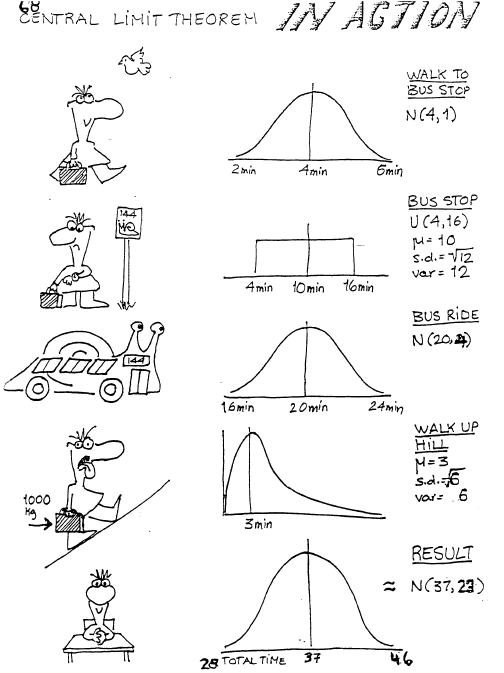
\includegraphics[width=\maxwidth]{/home/sahir/git_repositories/raqc/006-sensitivity-analysis-one-parameter/clt} 

\end{knitrout}


\FloatBarrier

\section{Proof of CLT in Action with \texttt{R} and \texttt{knitr::knit\_expand}}





\newpage
\subsection{$n$ = 10}

\begin{knitrout}
\definecolor{shadecolor}{rgb}{0.969, 0.969, 0.969}\color{fgcolor}\begin{figure}[h]

{\centering 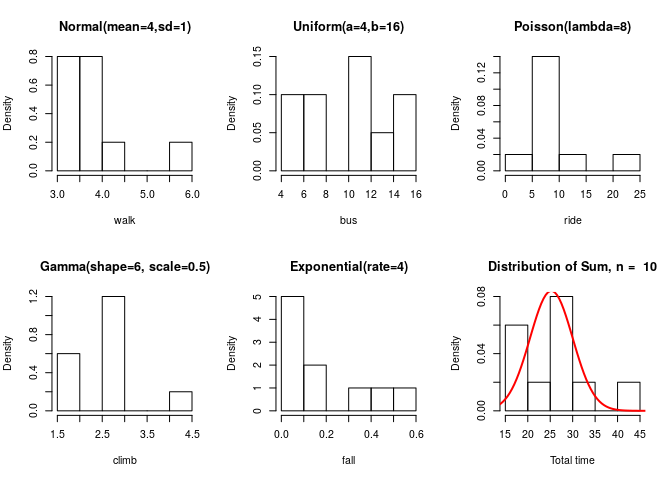
\includegraphics[width=\maxwidth]{figure/n-10-1} 

}

\caption[CLT in Action with $n$ = 10]{CLT in Action with $n$ = 10}\label{fig:n-10}
\end{figure}


\end{knitrout}
\newpage
\subsection{$n$ = 110}

\begin{knitrout}
\definecolor{shadecolor}{rgb}{0.969, 0.969, 0.969}\color{fgcolor}\begin{figure}[h]

{\centering 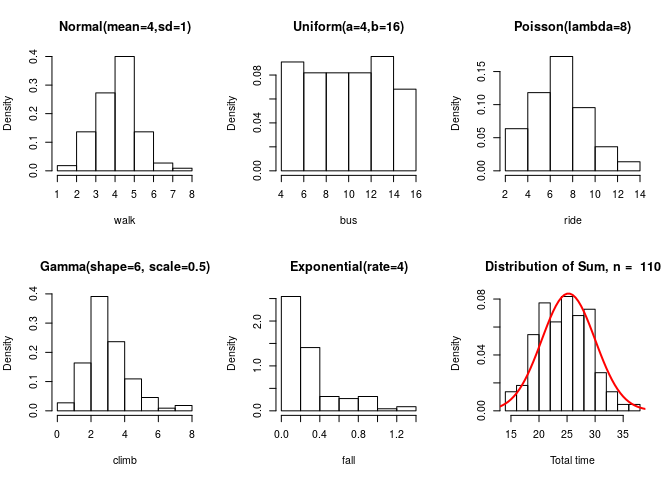
\includegraphics[width=\maxwidth]{figure/n-110-1} 

}

\caption[CLT in Action with $n$ = 110]{CLT in Action with $n$ = 110}\label{fig:n-110}
\end{figure}


\end{knitrout}
\newpage
\subsection{$n$ = 210}

\begin{knitrout}
\definecolor{shadecolor}{rgb}{0.969, 0.969, 0.969}\color{fgcolor}\begin{figure}[h]

{\centering 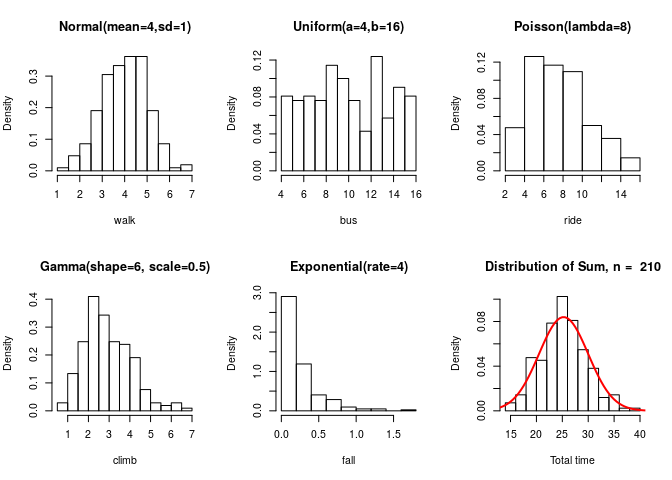
\includegraphics[width=\maxwidth]{figure/n-210-1} 

}

\caption[CLT in Action with $n$ = 210]{CLT in Action with $n$ = 210}\label{fig:n-210}
\end{figure}


\end{knitrout}
\newpage
\subsection{$n$ = 310}

\begin{knitrout}
\definecolor{shadecolor}{rgb}{0.969, 0.969, 0.969}\color{fgcolor}\begin{figure}[h]

{\centering 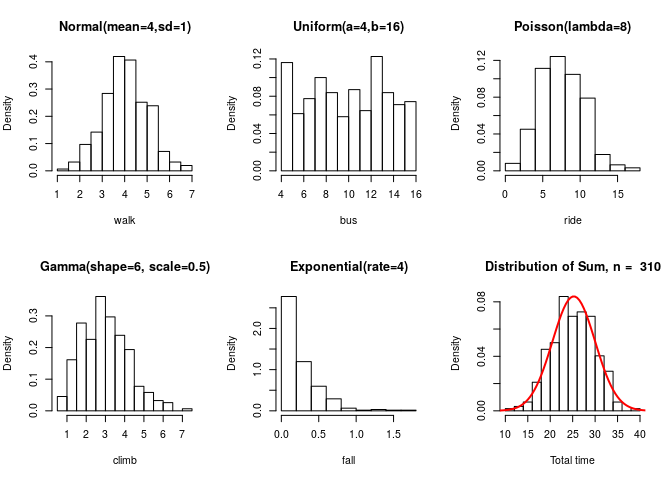
\includegraphics[width=\maxwidth]{figure/n-310-1} 

}

\caption[CLT in Action with $n$ = 310]{CLT in Action with $n$ = 310}\label{fig:n-310}
\end{figure}


\end{knitrout}
\newpage
\subsection{$n$ = 410}

\begin{knitrout}
\definecolor{shadecolor}{rgb}{0.969, 0.969, 0.969}\color{fgcolor}\begin{figure}[h]

{\centering 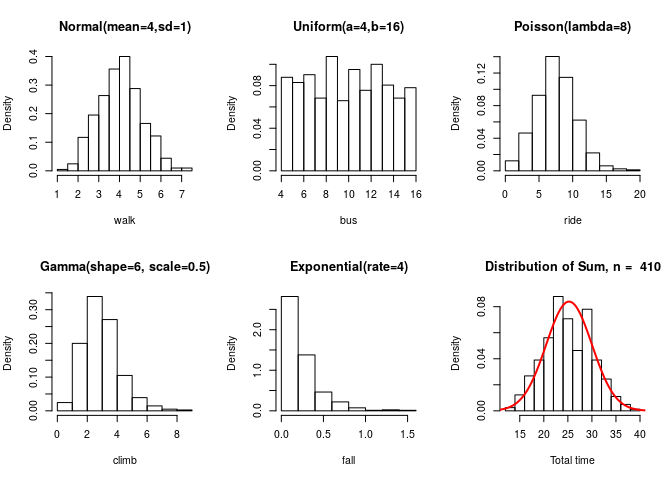
\includegraphics[width=\maxwidth]{figure/n-410-1} 

}

\caption[CLT in Action with $n$ = 410]{CLT in Action with $n$ = 410}\label{fig:n-410}
\end{figure}


\end{knitrout}
\newpage
\subsection{$n$ = 510}

\begin{knitrout}
\definecolor{shadecolor}{rgb}{0.969, 0.969, 0.969}\color{fgcolor}\begin{figure}[h]

{\centering 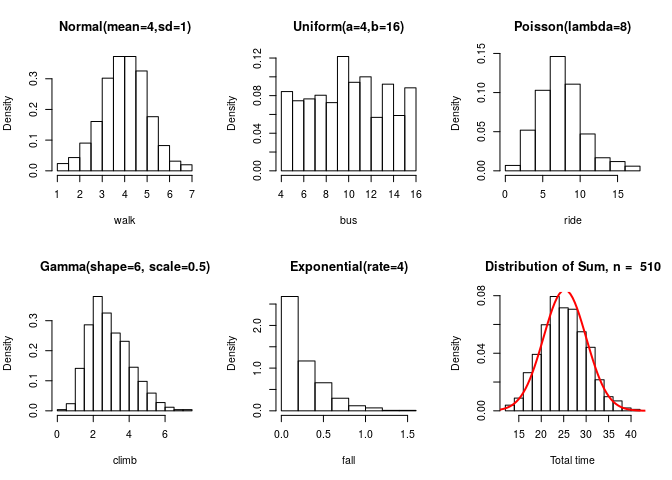
\includegraphics[width=\maxwidth]{figure/n-510-1} 

}

\caption[CLT in Action with $n$ = 510]{CLT in Action with $n$ = 510}\label{fig:n-510}
\end{figure}


\end{knitrout}
\newpage
\subsection{$n$ = 610}

\begin{knitrout}
\definecolor{shadecolor}{rgb}{0.969, 0.969, 0.969}\color{fgcolor}\begin{figure}[h]

{\centering 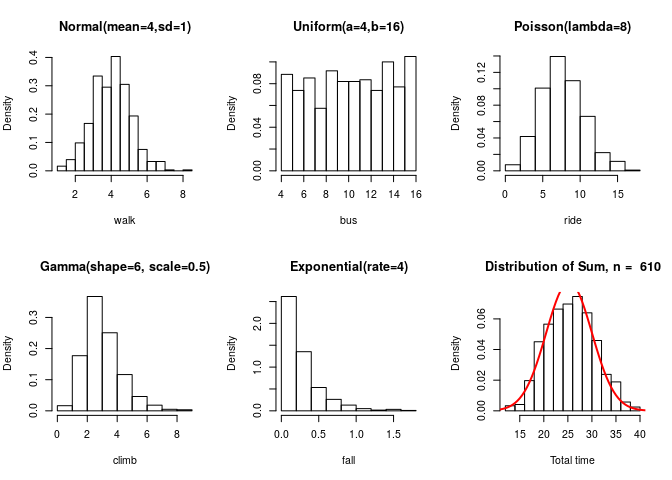
\includegraphics[width=\maxwidth]{figure/n-610-1} 

}

\caption[CLT in Action with $n$ = 610]{CLT in Action with $n$ = 610}\label{fig:n-610}
\end{figure}


\end{knitrout}
\newpage
\subsection{$n$ = 710}

\begin{knitrout}
\definecolor{shadecolor}{rgb}{0.969, 0.969, 0.969}\color{fgcolor}\begin{figure}[h]

{\centering 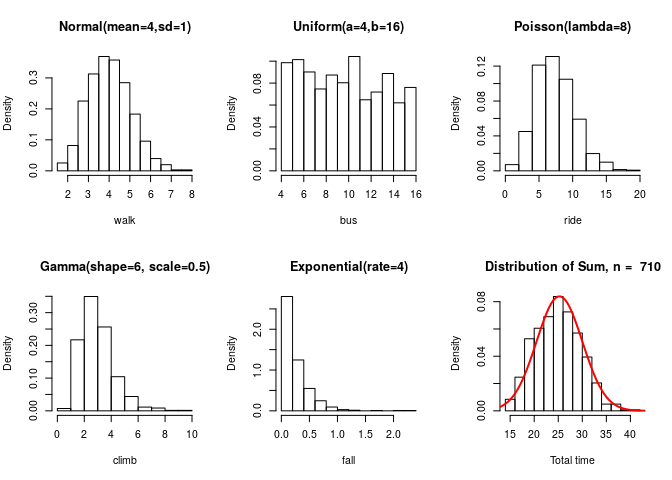
\includegraphics[width=\maxwidth]{figure/n-710-1} 

}

\caption[CLT in Action with $n$ = 710]{CLT in Action with $n$ = 710}\label{fig:n-710}
\end{figure}


\end{knitrout}
\newpage
\subsection{$n$ = 810}

\begin{knitrout}
\definecolor{shadecolor}{rgb}{0.969, 0.969, 0.969}\color{fgcolor}\begin{figure}[h]

{\centering 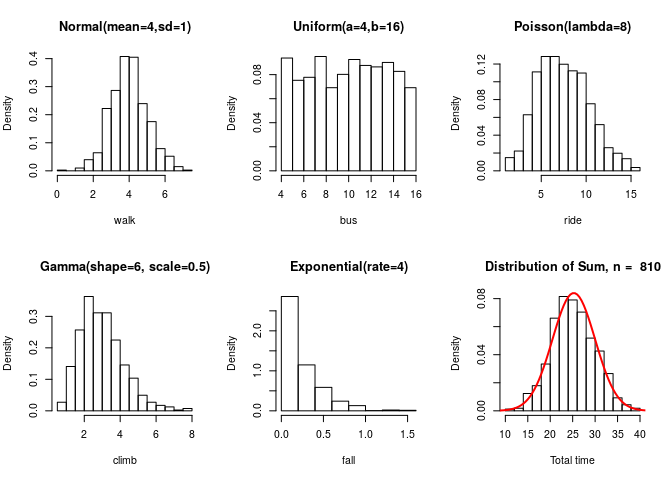
\includegraphics[width=\maxwidth]{figure/n-810-1} 

}

\caption[CLT in Action with $n$ = 810]{CLT in Action with $n$ = 810}\label{fig:n-810}
\end{figure}


\end{knitrout}
\newpage
\subsection{$n$ = 910}

\begin{knitrout}
\definecolor{shadecolor}{rgb}{0.969, 0.969, 0.969}\color{fgcolor}\begin{figure}[h]

{\centering 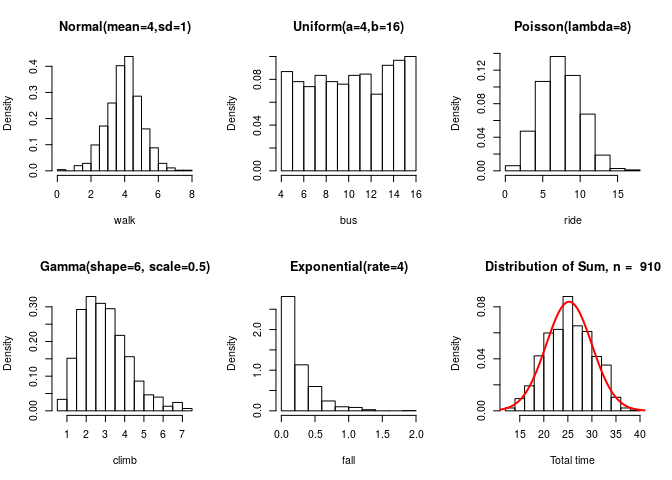
\includegraphics[width=\maxwidth]{figure/n-910-1} 

}

\caption[CLT in Action with $n$ = 910]{CLT in Action with $n$ = 910}\label{fig:n-910}
\end{figure}


\end{knitrout}
\newpage
\subsection{$n$ = 1010}

\begin{knitrout}
\definecolor{shadecolor}{rgb}{0.969, 0.969, 0.969}\color{fgcolor}\begin{figure}[h]

{\centering 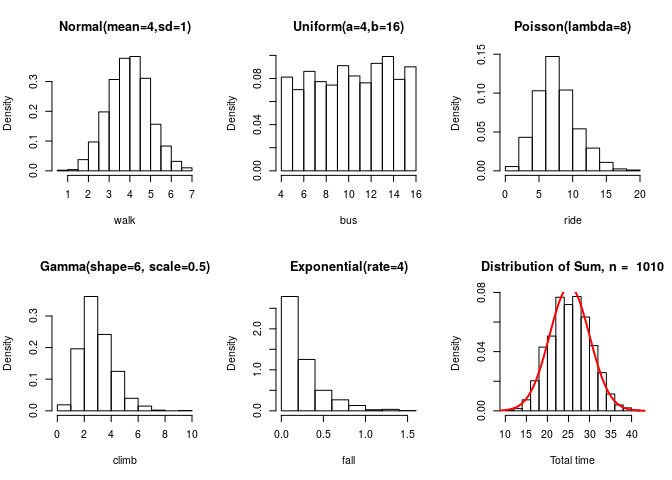
\includegraphics[width=\maxwidth]{figure/n-1010-1} 

}

\caption[CLT in Action with $n$ = 1010]{CLT in Action with $n$ = 1010}\label{fig:n-1010}
\end{figure}


\end{knitrout}
\newpage
\subsection{$n$ = 1110}

\begin{knitrout}
\definecolor{shadecolor}{rgb}{0.969, 0.969, 0.969}\color{fgcolor}\begin{figure}[h]

{\centering 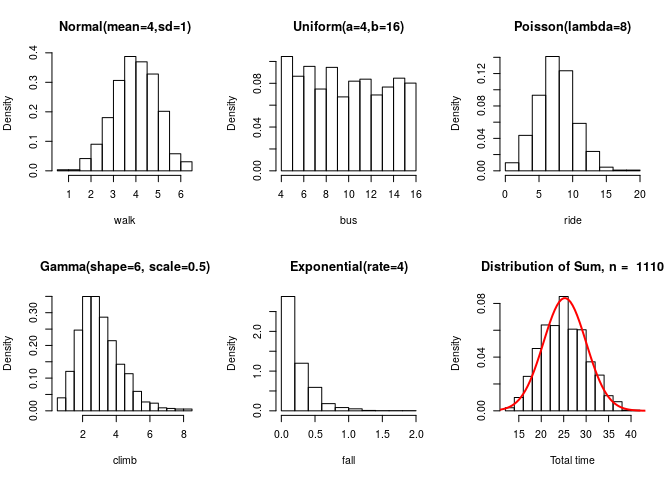
\includegraphics[width=\maxwidth]{figure/n-1110-1} 

}

\caption[CLT in Action with $n$ = 1110]{CLT in Action with $n$ = 1110}\label{fig:n-1110}
\end{figure}


\end{knitrout}
\newpage
\subsection{$n$ = 1210}

\begin{knitrout}
\definecolor{shadecolor}{rgb}{0.969, 0.969, 0.969}\color{fgcolor}\begin{figure}[h]

{\centering 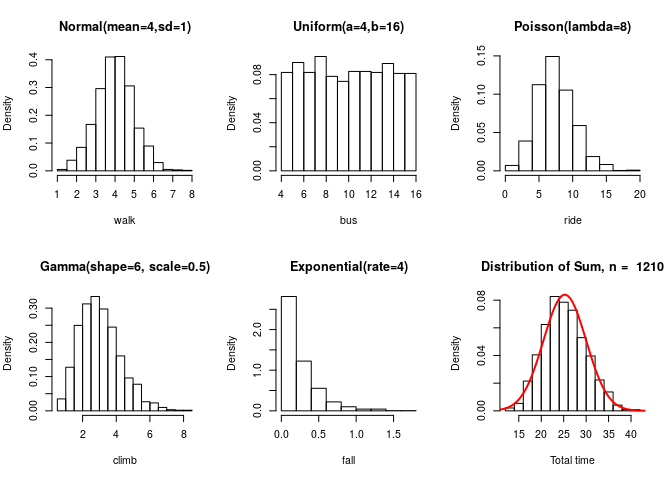
\includegraphics[width=\maxwidth]{figure/n-1210-1} 

}

\caption[CLT in Action with $n$ = 1210]{CLT in Action with $n$ = 1210}\label{fig:n-1210}
\end{figure}


\end{knitrout}
\newpage
\subsection{$n$ = 1310}

\begin{knitrout}
\definecolor{shadecolor}{rgb}{0.969, 0.969, 0.969}\color{fgcolor}\begin{figure}[h]

{\centering 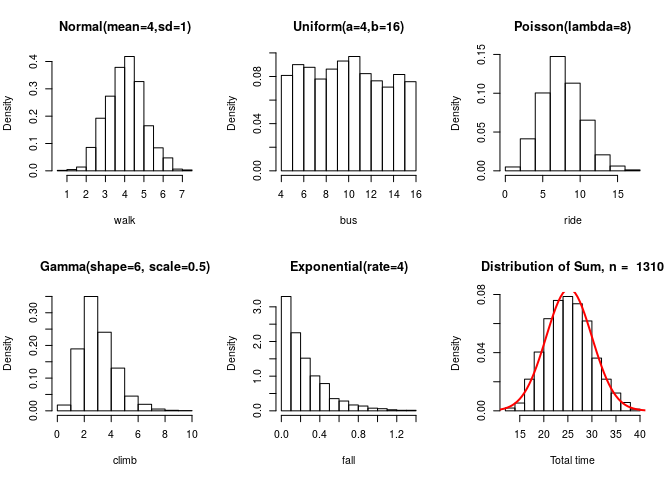
\includegraphics[width=\maxwidth]{figure/n-1310-1} 

}

\caption[CLT in Action with $n$ = 1310]{CLT in Action with $n$ = 1310}\label{fig:n-1310}
\end{figure}


\end{knitrout}
\newpage
\subsection{$n$ = 1410}

\begin{knitrout}
\definecolor{shadecolor}{rgb}{0.969, 0.969, 0.969}\color{fgcolor}\begin{figure}[h]

{\centering 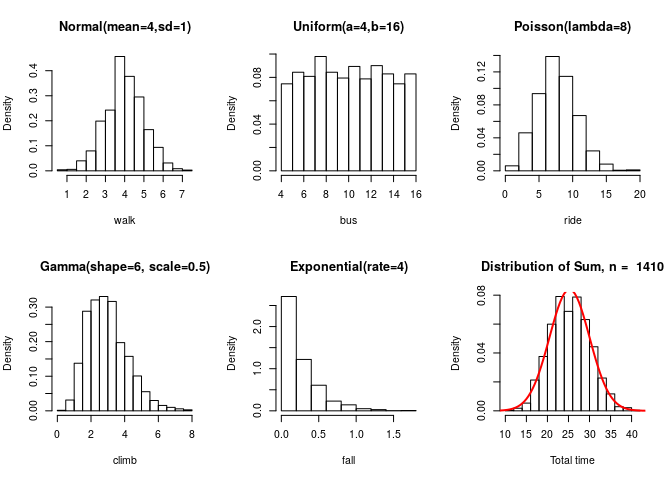
\includegraphics[width=\maxwidth]{figure/n-1410-1} 

}

\caption[CLT in Action with $n$ = 1410]{CLT in Action with $n$ = 1410}\label{fig:n-1410}
\end{figure}


\end{knitrout}
\newpage
\subsection{$n$ = 1510}

\begin{knitrout}
\definecolor{shadecolor}{rgb}{0.969, 0.969, 0.969}\color{fgcolor}\begin{figure}[h]

{\centering 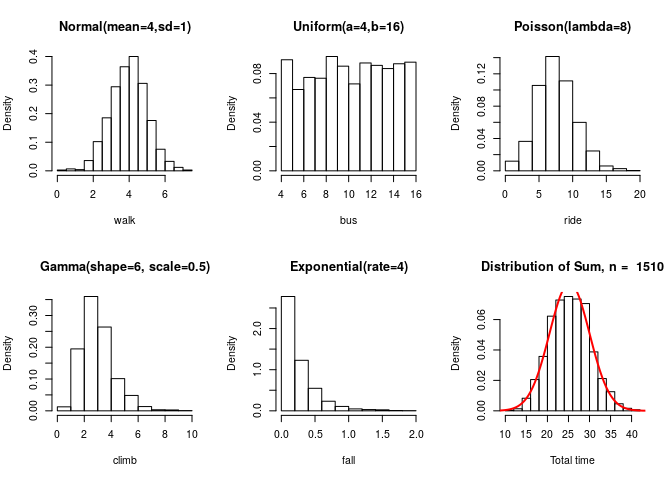
\includegraphics[width=\maxwidth]{figure/n-1510-1} 

}

\caption[CLT in Action with $n$ = 1510]{CLT in Action with $n$ = 1510}\label{fig:n-1510}
\end{figure}


\end{knitrout}
\newpage
\subsection{$n$ = 1610}

\begin{knitrout}
\definecolor{shadecolor}{rgb}{0.969, 0.969, 0.969}\color{fgcolor}\begin{figure}[h]

{\centering 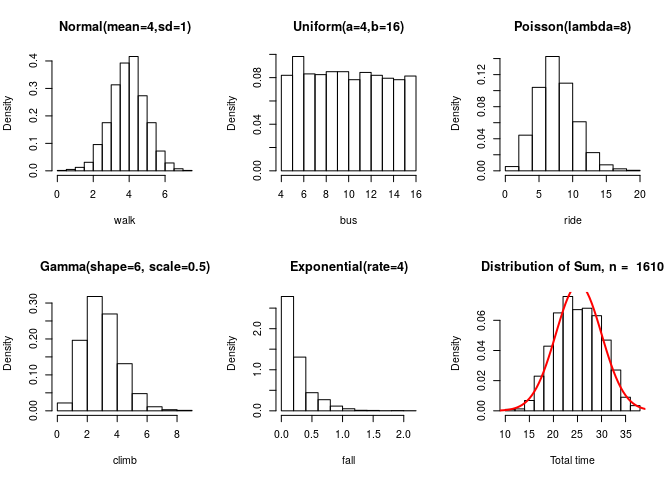
\includegraphics[width=\maxwidth]{figure/n-1610-1} 

}

\caption[CLT in Action with $n$ = 1610]{CLT in Action with $n$ = 1610}\label{fig:n-1610}
\end{figure}


\end{knitrout}
\newpage
\subsection{$n$ = 1710}

\begin{knitrout}
\definecolor{shadecolor}{rgb}{0.969, 0.969, 0.969}\color{fgcolor}\begin{figure}[h]

{\centering 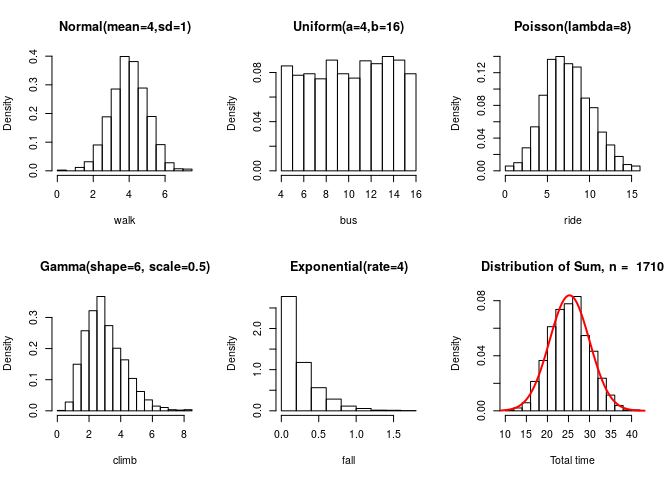
\includegraphics[width=\maxwidth]{figure/n-1710-1} 

}

\caption[CLT in Action with $n$ = 1710]{CLT in Action with $n$ = 1710}\label{fig:n-1710}
\end{figure}


\end{knitrout}
\newpage
\subsection{$n$ = 1810}

\begin{knitrout}
\definecolor{shadecolor}{rgb}{0.969, 0.969, 0.969}\color{fgcolor}\begin{figure}[h]

{\centering 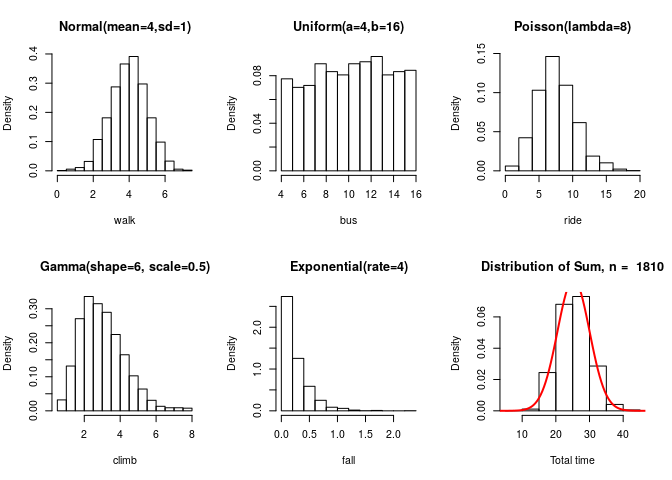
\includegraphics[width=\maxwidth]{figure/n-1810-1} 

}

\caption[CLT in Action with $n$ = 1810]{CLT in Action with $n$ = 1810}\label{fig:n-1810}
\end{figure}


\end{knitrout}
\newpage
\subsection{$n$ = 1910}

\begin{knitrout}
\definecolor{shadecolor}{rgb}{0.969, 0.969, 0.969}\color{fgcolor}\begin{figure}[h]

{\centering 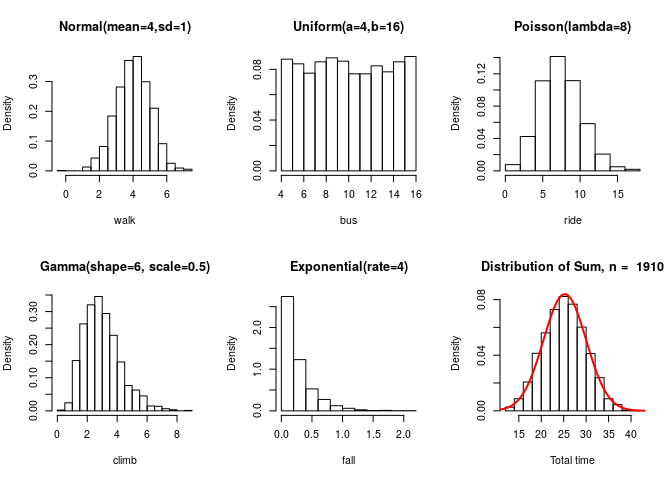
\includegraphics[width=\maxwidth]{figure/n-1910-1} 

}

\caption[CLT in Action with $n$ = 1910]{CLT in Action with $n$ = 1910}\label{fig:n-1910}
\end{figure}


\end{knitrout}
\newpage
\subsection{$n$ = 2010}

\begin{knitrout}
\definecolor{shadecolor}{rgb}{0.969, 0.969, 0.969}\color{fgcolor}\begin{figure}[h]

{\centering 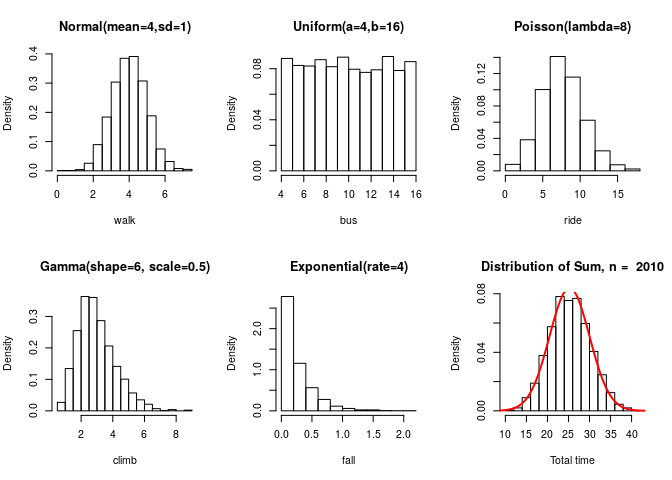
\includegraphics[width=\maxwidth]{figure/n-2010-1} 

}

\caption[CLT in Action with $n$ = 2010]{CLT in Action with $n$ = 2010}\label{fig:n-2010}
\end{figure}


\end{knitrout}



\FloatBarrier
\bibliography{006-bibliography}

\newpage
\appendix
\section{Session Information}
\begin{knitrout}
\definecolor{shadecolor}{rgb}{0.969, 0.969, 0.969}\color{fgcolor}\begin{kframe}
\begin{alltt}
\hlkwd{print}\hlstd{(}\hlkwd{sessionInfo}\hlstd{(),} \hlkwc{locale} \hlstd{=} \hlnum{FALSE}\hlstd{)}
\end{alltt}
\begin{verbatim}
## R version 3.6.0 (2019-04-26)
## Platform: x86_64-pc-linux-gnu (64-bit)
## Running under: Pop!_OS 18.10
## 
## Matrix products: default
## BLAS:   /usr/lib/x86_64-linux-gnu/blas/libblas.so.3.8.0
## LAPACK: /usr/lib/x86_64-linux-gnu/lapack/liblapack.so.3.8.0
## 
## attached base packages:
## [1] stats     graphics  grDevices utils     datasets 
## [6] methods   base     
## 
## other attached packages:
## [1] here_0.1     pacman_0.5.0 knitr_1.22  
## 
## loaded via a namespace (and not attached):
##  [1] compiler_3.6.0  backports_1.1.3 magrittr_1.5   
##  [4] rprojroot_1.3-2 formatR_1.6     tools_3.6.0    
##  [7] stringi_1.4.3   stringr_1.4.0   xfun_0.6       
## [10] evaluate_0.13
\end{verbatim}
\end{kframe}
\end{knitrout}


\end{document}
